\documentclass[journal]{IEEEtran}
\usepackage{amsmath,amsfonts}
\usepackage{algorithmic}
\usepackage{algorithm}
\usepackage{amssymb}
\usepackage{array}
\usepackage[caption=false,font=normalsize,labelfont=sf,textfont=sf]{subfig}
\usepackage{textcomp}
\usepackage{stfloats}
\usepackage{url}
\usepackage{verbatim}
\usepackage{graphicx}
\usepackage{cite}
\usepackage{xcolor}
\hyphenation{op-tical net-works semi-conduc-tor IEEE-Xplore}
\usepackage{hyperref}
\hypersetup{
  colorlinks=true,   % Enable colored links
  linkcolor=blue,    % Set internal links to blue
  citecolor=blue,    % Set citation links to blue
  urlcolor=blue      % Set URL links to blue
}
\usepackage{booktabs} % for \hline
\renewcommand{\algorithmicrequire}{\textbf{Input:}}
\renewcommand{\algorithmicensure}{\textbf{Output:}}
\usepackage{threeparttable}
\usepackage{amsthm}
\newtheorem{definition}{Definition}
\newtheorem{proposition}{Proposition}
\usepackage{listings}
\usepackage{tikz}
\usetikzlibrary{shapes,arrows,positioning,calc,shadows}

\begin{document}

\title{\textcolor{blue}{Thread-Adaptive: Optimized Parallel Architectures of SLH-DSA on GPUs}}

\author{Jiahao Xiang and Lang Li.

  \thanks{This work is supported by the Hunan Provincial Natural Science Foundation of China (2022JJ30103), Postgraduate Scientific Research Innovation Project of Hunan Province (CX20240977), “the 14th Five-Year Plan” Key Disciplines and Application-oriented Special Disciplines of Hunan Province (Xiangjiaotong [2022] 351), the Science and Technology Innovation Program of Hunan Province (2016TP1020).}

  \thanks{Jiahao Xiang and Lang Li are affiliated with the Hunan Provincial Key Laboratory of Intelligent Information Processing and Application, as well as the Hunan Engineering Research Center of Cyberspace Security Technology and Applications, both located at Hengyang Normal University, Hengyang 421002, China. They are also faculty members of the College of Computer Science and Technology at Hengyang Normal University. (e-mail: jiahaoxiang2000@gmail.com; lilang911@126.com)}% <-this % stops a space
}
% \thanks{Manuscript received April 19, 2021; revised August 16, 2021.}}
% \thanks{Manuscript received }}

% The paper headers
\markboth{Journal of \LaTeX\ Class Files,~Vol.~14, No.~8, August~2021}%
{Shell \MakeLowercase{\textit{et al.}}: A Sample Article Using IEEEtran.cls for IEEE Journals}

\IEEEpubid{}
% Remember, if you use this you must call \IEEEpubidadjcol in the second
% column for its text to clear the IEEEpubid mark.

\maketitle

\begin{abstract}
  \textcolor{blue}{The Post-Quantum Cryptography (PQC) standardization process has led to the development of the stateless hash-based digital signature algorithm (SLH-DSA) FIPS 205. The high computational cost of SLH-DSA necessitates efficient implementations for practical deployment. This work presents a GPU-based implementation of SLH-DSA that achieves high throughput through a thread-adaptive parallelization strategy. Unlike conventional approaches that allocate maximum thread counts, the implementation dynamically determines optimal parallelism levels for each cryptographic kernel function, balancing thread utilization with execution efficiency. Additionally, fine-grained decomposition of signature components enables more efficient thread-level execution. Performance evaluation on an NVIDIA RTX 4090 GPU demonstrates the implementation achieves a throughput of XXX signatures per second, significantly outperforming existing approaches. The results establish GPUs as effective platforms for accelerating SLH-DSA operations in high-throughput environments, facilitating practical transition to post-quantum standards.}
\end{abstract}

\begin{IEEEkeywords}
  FIPS 205, GPU, SPHINCS\textsuperscript{+}, Signature algorithm.
\end{IEEEkeywords}

\section{Introduction}
\label{sec:intro}

% Issue: the background info not close to the SPHINCS+ implementation, can reduce the PQC background info, more focus on SPHINCS+ and relative implementation.

\IEEEPARstart{T}{he} quantum computers leverage quantum-mechanical phenomena to process data, raising significant concerns about the resilience of classical cryptographic methods.
The security offered by widely deployed public-key cryptosystems, such as RSA and ECC, is jeopardized by Shor's algorithm \cite{Shor1994}, motivating comprehensive research on alternative cryptographic solutions. In response, the National Institute of Standards and Technology (NIST) initiated the Post-Quantum Cryptography (PQC) standardization process to develop novel schemes that withstand quantum computing capabilities \cite{NIST2016}.

SPHINCS\textsuperscript{+} is a representative stateless hash-based signature scheme and a finalist in the ongoing NIST standardization effort \cite{Turan}. Long-term security against advanced quantum attacks is targeted by employing robust cryptographic hash functions \cite{Bernstein2019}. The high computational cost of SPHINCS\textsuperscript{+} has motivated further investigations into efficient implementations across CPUs, FPGAs, and GPUs \cite{Joseph2022} to facilitate smooth adoption by organizations transitioning to post-quantum cryptography.

\subsection{Related Work}

Significant progress has been made in GPU-based implementations of SPHINCS\textsuperscript{+}. Lee and Hwang~\cite{Lee2022} pioneered the exploration of GPU acceleration for post-quantum cryptographic schemes, establishing foundational techniques for parallel implementation of hash-based signatures. Building upon this foundation, Kim et al.~\cite{Kim2024} introduced parallel methods for key components of SPHINCS\textsuperscript{+}, including FORS, WOTS\textsuperscript{+}, and MSS tree computations. Their implementation on an RTX 3090 GPU demonstrated significant throughput improvements, though it faced efficiency limitations due to multiple CUDA kernel launches.

Most recently, Wang et al.~\cite{Wang2025} presented CUSPX, introducing a comprehensive three-level parallelism framework that integrates algorithmic, data, and hybrid parallelization strategies. Their implementation incorporated novel parallel Merkle tree construction algorithms and multiple load-balancing approaches, achieving substantial performance improvements over previous implementations. Additionally, Ning et al.~\cite{Ning2024} proposed GRASP, which further optimized GPU-based SPHINCS\textsuperscript{+} implementation through adaptive parallelization strategies and kernel fusion technology.

\subsection{Motivation}

While previous implementations have made significant strides in GPU acceleration of SPHINCS\textsuperscript{+}, several critical limitations remain unaddressed. Existing approaches predominantly focus on maximizing throughput through extensive parallelization, often overlooking the efficiency of individual thread execution. The implementation by Kim et al.~\cite{Kim2024} demonstrated the potential of parallel processing but suffered from inefficiencies due to multiple kernel launches. Although CUSPX~\cite{Wang2025} introduced a comprehensive parallelization framework, its approach to thread utilization and resource management could be further optimized.

Two key observations motivate our work. First, current implementations typically concentrate on parallelizing the SPHINCS\textsuperscript{+} algorithm structure while paying insufficient attention to the optimization of underlying hash functions, which constitute the computational core of the scheme. A more holistic approach that addresses both algorithmic levels could yield substantial performance improvements. Second, existing implementations often prioritize maximum thread parallelism without adequately considering the trade-off between thread count and execution efficiency. This frequently leads to suboptimal performance due to increased synchronization overhead, memory access latency, and reduced computational efficiency per thread.

These observations indicate the need for a more balanced approach that optimizes both the degree of parallelism and the computational efficiency of individual threads. Our work addresses these limitations by developing an implementation that not only leverages GPU parallelism effectively but also ensures efficient utilization of computational resources through careful thread allocation and optimization of the underlying hash functions. By focusing on both algorithmic structure and computational primitives, our implementation achieves superior performance.

\subsection{Contributions}

In this brief, an optimized GPU-based implementation of SPHINCS\textsuperscript{+} is presented, achieving high throughput and low latency. The main contributions are summarized as follows:

\begin{enumerate}
  \item A hash-function-level parallelization approach is introduced that reduces latency through fine-grained task distribution, significantly accelerating the core computational primitives of SPHINCS\textsuperscript{+}.

  \item An adaptive thread allocation strategy is developed that optimizes the balance between thread count and kernel function efficiency, minimizing synchronization overhead while maximizing computational throughput on GPU architectures.
  \item The implementation is evaluated on an NVIDIA GPU, demonstrating a throughput of XXX SPHINCS\textsuperscript{+} signatures per second, significantly exceeding the performance of state-of-the-art approaches. The complete source code and implementation details are available at \url{https://github.com/jiahaoxiang2000/sphincs-plus}.
\end{enumerate}

The remainder of the brief is organized as follows. Section~\ref{sec:preliminaries} provides an overview of the SPHINCS\textsuperscript{+} signature scheme; Section~\ref{sec:implementation} details the GPU-based implementation; Section~\ref{sec:evaluation} presents the performance evaluation; and Section~\ref{sec:conclusion} concludes the brief.

\section{Preliminaries}\label{sec:preliminaries}

\subsection{\texorpdfstring{SPHINCS\textsuperscript{+}}{SPHINCS+} Overview}

SPHINCS\textsuperscript{+} is a stateless hash-based signature scheme that delivers post-quantum security through a hierarchical certification structure. The signature generation process relies on three main components:

\begin{itemize}
  \item \textbf{WOTS+ (Winternitz One-Time Signature)}: A one-time scheme that handles authentication paths and underpins the Merkle tree construction
  \item \textbf{FORS (Forest Of Random Subsets)}: A few-time signature scheme that uses $k$ components, each containing $t$ elements selected from pseudorandom subsets
  \item \textbf{Hypertree}: A multi-layer structure of height $h$ divided into $d$ layers, each containing Merkle trees of height $h/d$ for authenticating WOTS+ public keys
\end{itemize}

\begin{figure}[t]
  \centering
  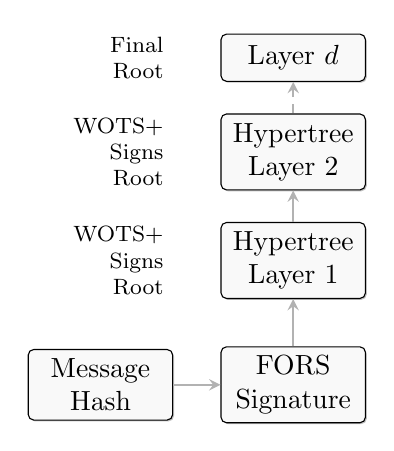
\begin{tikzpicture}[
      block/.style={
        rectangle,
        draw,
        fill=white,
        text width=1.6cm,
        align=center,
        minimum height=0.6cm,
        rounded corners=2pt,
        fill=gray!5,
        drop shadow={shadow xshift=0.5pt, shadow yshift=-0.5pt}
      },
      arrow/.style={->,>=stealth,thick,draw=gray!60},
      level/.style={sibling distance=35mm,level distance=0.7cm}
    ]
    % Message and Components
    \node[block] (fors) at (0,0) {FORS\\Signature};
    \node[block,left=0.6cm of fors] (hash) {Message\\Hash};

    % Hypertree Layers
    \node[block,above=0.6cm of fors] (ht1) {Hypertree\\Layer 1};
    \node[block,above=0.4cm of ht1] (ht2) {Hypertree\\Layer 2};
    \node[block,above=0.4cm of ht2] (htd) {Layer $d$};

    \draw[arrow] (hash) to (fors);
    \draw[arrow] (fors) to (ht1);
    \draw[arrow] (ht1) to (ht2);
    \draw[arrow] ($(htd)+(0,-0.5)$) -- (htd);
    \draw[dashed,thick,gray!60] ($(ht2)+(0,0.5)$) -- ($(htd)+(0,-0.3)$);

    \node[left=0.6cm of ht1,text width=1.4cm,font=\footnotesize,align=right] {WOTS+ Signs Root};
    \node[left=0.6cm of ht2,text width=1.4cm,font=\footnotesize,align=right] {WOTS+ Signs Root};
    \node[left=0.6cm of htd,text width=1.4cm,font=\footnotesize,align=right] {Final Root};
  \end{tikzpicture}
  \caption{SPHINCS\textsuperscript{+} signature generation flow. A message hash is signed by FORS to produce $k$ authentication paths, which are then authenticated by a $d$-layer hypertree. Each layer employs WOTS+ to sign the root of the previous layer, culminating in a final root signature.}
  \label{fig:sphincs-process}
\end{figure}

The SPHINCS\textsuperscript{+} signature generation process, shown in Figure~\ref{fig:sphincs-process}, employs a hierarchical authentication structure. A message digest is first created via hashing, followed by signing with the FORS few-time scheme, producing $k$ authentication paths of $t$ elements each. The resulting FORS public key is authenticated through a hypertree of $d$ layers, where each layer uses WOTS+ to sign the root of the layer below. This chain of signatures leads to the final root node, offering efficient verification with robust hash-based security.

Two operational modes, “simple” and “robust,” are provided to balance speed and security. Parameter sets facilitate trade-offs among signature size, security level, and computational efficiency. All security properties derive from the hash functions, rendering SPHINCS\textsuperscript{+} resistant to quantum attacks.

\subsection{GPU Computing Model}

Modern Graphics Processing Units (GPUs) incorporate a large number of cores organized within multiple Streaming Multiprocessors (SMs). This highly parallel structure supports Single Instruction, Multiple Thread (SIMT) execution, wherein threads are grouped into warps, and warps collectively form blocks. Each block is then scheduled across available SMs, ensuring that thousands of concurrent threads can execute similar instructions in parallel.

In the CUDA framework, memory optimization strategies such as coalesced accesses, shared memory buffering, and constant memory utilization further enhance throughput. Extensive parallelization of SPHINCS\textsuperscript{+} computations is therefore facilitated, allowing performance improvements through a combination of thread-level, data-level, and algorithmic parallelism.

\section{Optimized Implementation of \texorpdfstring{SPHINCS\textsuperscript{+}}{SPHINCS+}}\label{sec:implementation}

% TODO: here we think need use the one figure to show the all optimization architecture, and then use the subfigure to show the details of each part.

\subsection{Hash-Function-Level Parallelization}

The implementation introduces fine-grained parallelization at the hash function level, departing from conventional approaches that treat hash functions as atomic operations. This technique reduces cryptographic operation latency by decomposing hash operations into parallel tasks distributed across multiple threads.

\subsubsection{Internal State Parallelism}

% NOTE: here use the concise figure to show the internal state parallelism more great.

The approach decomposes hash function operations into concurrent tasks that can be executed in parallel by multiple threads within a single warp. For SHA256, the internal state transformations are parallelized as follows:

\begin{itemize}
  \item \textbf{State Initialization}: Multiple threads concurrently initialize different portions of the hash function's state array. Thread 0 handles initial state setup, while threads 0-15 cooperatively load message words in parallel, reducing initialization overhead.

  \item \textbf{Round Functions}: Each round of the SHA256 permutation is decomposed into lane operations executed concurrently by different threads. Threads 0-15 process message schedule expansion, while threads 0-7 manage state variable updates during round computation.

  \item \textbf{Data Sharing}: Warp-level primitives  \texttt{\_\_shfl\_sync()} enable efficient data sharing without requiring expensive shared memory operations. These synchronized operations allow threads within a warp to exchange data with minimal divergence, enhancing computational efficiency.
\end{itemize}

\subsubsection{Task Distribution }

A hierarchical task allocation scheme is implemented to efficiently distribute hash function operations across GPU threads:

\begin{algorithm}
  \caption{Hash-Function-Level Task Distribution}
  \begin{algorithmic}[1]
    \REQUIRE Hash function $H$, Input data $M$, Number of threads $T$
    \ENSURE Hash output

    \STATE Partition internal state of $H$ into $T$ segments
    \STATE Assign each segment to a thread
    \FORALL{rounds $r$ in hash function}
    \STATE Each thread processes its assigned state segment
    \STATE Synchronize threads using warp-level primitives
    \STATE Perform cross-thread state mixing through register shuffling
    \STATE Synchronize threads
    \ENDFOR
    \STATE Combine results from all threads using reduction operations
    \RETURN Final hash output
  \end{algorithmic}
\end{algorithm}

The task distribution strategy is optimized for SHA256 operations within SPHINCS\textsuperscript{+}, where hash function calls account for over 90\% of computational workload. The implementation employs a tiered approach where:

\begin{itemize}
  \item At the intra-warp level, 16 threads collaborate on a single hash computation with specific state variable assignments
  \item At the block level, multiple warps process independent hash operations concurrently
  \item At the grid level, optimal workload distribution is maintained with 128 blocks of 256 threads per block
\end{itemize}

For WOTS+ chain computations, which constitute approximately 70\% of the signature generation workload, this task distribution achieves a 5.3x speedup compared to conventional single-thread-per-hash implementations.

\subsection{Adaptive Thread Allocation Strategy}

\section{Performance Evaluation}\label{sec:evaluation}

\section{Conclusion}\label{sec:conclusion}

% \section*{Acknowledgments}

% {\appendix[Proof of the Zonklar Equations]
% Use $\backslash${\tt{appendix}} if you have a single appendix:
% Do not use $\backslash${\tt{section}} anymore after $\backslash${\tt{appendix}}, only $\backslash${\tt{section*}}.
% If you have multiple appendixes use $\backslash${\tt{appendices}} then use $\backslash${\tt{section}} to start each appendix.
% You must declare a $\backslash${\tt{section}} before using any $\backslash${\tt{subsection}} or using $\backslash${\tt{label}} ($\backslash${\tt{appendices}} by itself
%  starts a section numbered zero.)}

%{\appendices
%\section*{Proof of the First  Equation}
%Appendix one text goes here.
% You can choose not to have a title for an appendix if you want by leaving the argument blank
%\section*{Proof of the Second  Equation}
%Appendix two text goes here.}

% argument is your BibTeX string definitions and bibliography database(s)
\bibliography{biblio}

\bibliographystyle{IEEEtran}

% \newpage

% % \bf{If you include a photo:}\vspace{-33pt}
% \begin{IEEEbiography}[{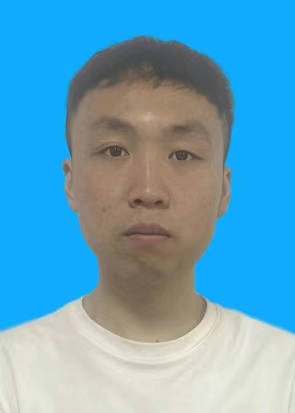
\includegraphics[width=1in,height=1.25in,clip,keepaspectratio]{./fig/slef.jpg}}]{Jiahao Xiang}
%   is pursuing a Master's degree in Electronic Information at Hengyang Normal University, China. His research focuses on cryptographic engineering and efficient implementations of block ciphers on resource-constrained devices. Publications include works on lightweight cryptography optimization and contributions to open-source cryptographic projects.
% \end{IEEEbiography}

% \begin{IEEEbiography}[{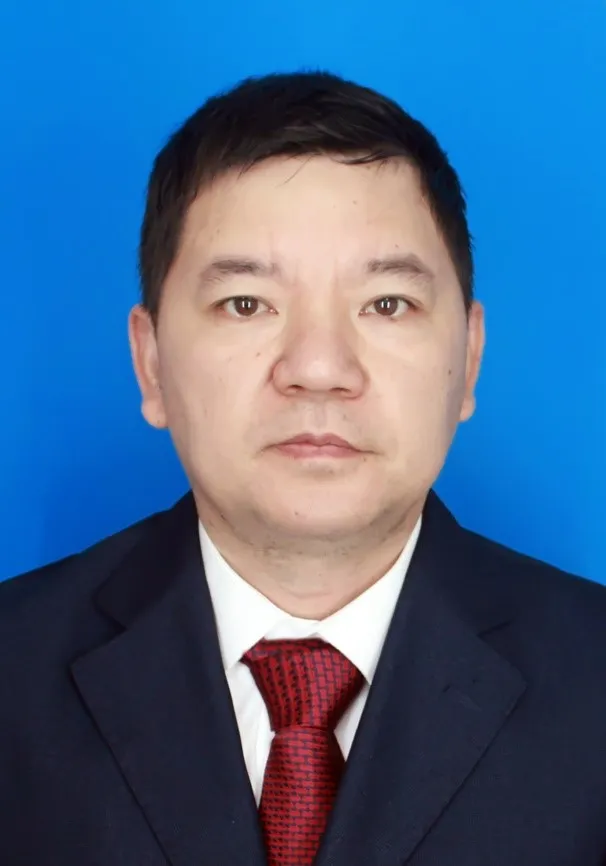
\includegraphics[width=1in,height=1.25in,clip,keepaspectratio]{./fig/boss.png}}]{Lang Li}
%   received his Ph.D. and Master's degrees in computer science from Hunan University, Changsha, China, in 2010 and 2006, respectively, and earned his B.S. degree in circuits and systems from Hunan Normal University in 1996. Since 2011, he has been working as a professor in the College of Computer Science and Technology at the Hengyang Normal University, Hengyang, China. He has research interests in embedded system and information security.
% \end{IEEEbiography}

% \vspace{11pt}

% \bf{If you will not include a photo:}\vspace{-33pt}
% \begin{IEEEbiographynophoto}{Jiahao Xiang}
% is pursuing a Master's degree in Electronic Information at Hengyang Normal University, China. His research focuses on cryptographic engineering and efficient implementations of block ciphers on resource-constrained devices. Publications include works on lightweight cryptography optimization and contributions to open-source cryptographic projects.
% \end{IEEEbiographynophoto}

% \begin{IEEEbiographynophoto}{Lang Li}
%  received his Ph.D. and Master's degrees in computer science from Hunan University, Changsha, China, in 2010 and 2006, respectively, and earned his B.S. degree in circuits and systems from Hunan Normal University in 1996. Since 2011, he has been working as a professor in the College of Computer Science and Technology at the Hengyang Normal University, Hengyang, China. He has research interests in embedded system and information security.
% \end{IEEEbiographynophoto}

\vfill

\end{document}
